\documentclass[11pt,a4paper]{article}
\usepackage[utf8]{inputenc}
\usepackage[T1]{fontenc}
\usepackage{lmodern}
\usepackage{geometry}
\usepackage{graphicx}
\usepackage{float}
\usepackage{booktabs}
\usepackage{amsmath}
\usepackage{hyperref}
\geometry{margin=2.2cm}

\title{g4play: Geometry, Simulation Flow, and NN PID Model}
\author{Project documentation}
\date{\today}

\begin{document}
\maketitle

\section{Geant4 geometry model}
The detector model is implemented in \texttt{src/waterCherenkovSim.cpp}. The setup consists of:
\begin{itemize}
  \item World volume: air box (\(3\times 3\times 4\) m half-lengths).
  \item Cylindrical stainless-steel tank: outer radius \(1.75\) m, half-height \(2.0\) m.
  \item Steel wall/cap thickness: \(4\) mm.
  \item Inner water volume: radius \(1.75\text{ m} - 4\text{ mm}\), half-height \(2.0\text{ m} - 4\text{ mm}\).
\end{itemize}

Water optical properties use tabulated refractive index and absorption length versus photon energy. Air and vacuum are assigned optical refractive index tables for optical transport compatibility.

\subsection{Photosensor model}
Sensors are hemisphere modules covering barrel and endcaps:
\begin{itemize}
  \item Outer dome radius \(4\) cm, glass thickness \(1\) mm.
  \item Internal vacuum half-sphere.
  \item Silicon disk at the base: thickness \(5\) mm, radius \(3.8\) cm.
  \item Placement pitch: approximately \(10\) cm.
  \item Sensors are oriented inward; barrel placement leaves \(10\) cm clearance near endcaps.
\end{itemize}

The silicon optical surface is configured as an ideal absorber (\texttt{REFLECTIVITY=0}, \texttt{EFFICIENCY=1}), so each optical photon reaching the silicon is registered.

\section{Simulation call structure and momentum scan workflow}

\subsection{Single executable}
The CMake build generates:
\begin{verbatim}
./bin/waterCherenkovSim
\end{verbatim}
Macro files are stored under \texttt{configs/}.

\subsection{Momentum list scan (\texttt{run\_scan.py})}
\texttt{run\_scan.py} reads \texttt{configs/run.mac}, then for each requested momentum:
\begin{enumerate}
  \item rewrites \texttt{/gun/particle},
  \item rewrites \texttt{/gun/momentumAmp <P> MeV},
  \item writes a temporary macro file,
  \item runs:
\begin{verbatim}
source <geant4.sh> && exec ./bin/waterCherenkovSim <temp_macro>
\end{verbatim}
  \item stores output ROOT as
\begin{verbatim}
events_<particleTag>_p<P>MeV_<NeventsTag>[suffixes].root
\end{verbatim}
\end{enumerate}

Default momentum list:
\[
[200,250,300,350,400,450,500,550,600,650,700,750,800]\ \text{MeV}/c
\]

Geant4 environment script selection:
\begin{itemize}
  \item host \texttt{jirikvita}: \texttt{/home/qitek/install/geant4-v11.1.1-install/bin/geant4.sh}
  \item otherwise: \texttt{/home/qitek/work/g4/geant4-v11.1.2-install/bin/geant4.sh}
\end{itemize}

\subsection{Parallel particle scans (\texttt{superRun.py})}
\texttt{superRun.py} launches multiple \texttt{run\_scan.py} processes in parallel (default particles: \(e^+\), \(\mu^+\), \(\pi^+\)). Each process scans the same momentum list (or user-provided list).

\section{Poisson smearing and noise model}
Readout controls:
\begin{verbatim}
/g4play/silicon/smearPoissonHits true|false
/g4play/silicon/addNoise true|false
/g4play/silicon/noiseNu <nu>
\end{verbatim}

Per module, if raw detected count is \(N\):
\begin{itemize}
  \item if smearing enabled: \(N \leftarrow \mathrm{Poisson}(N)\),
  \item if additive noise enabled: \(N \leftarrow N + \mathrm{Poisson}(\nu)\), where \(\nu=\) \texttt{noiseNu}.
\end{itemize}

Output filename tags:
\begin{itemize}
  \item \texttt{\_PoissSmear} if smearing is enabled,
  \item \texttt{\_addNoise<nu>} if additive noise is enabled.
\end{itemize}

\section{NN architecture and hyperparameters}
The NN training pipeline is in \texttt{trainNN.py} and feature extraction in \texttt{pid\_features.py}.

\subsection{Input features}
For each event, the code aggregates statistics from vector branches in \texttt{silicon} and optional \texttt{muonDecay} tree:
\begin{itemize}
  \item count/sum/mean/std/min/max per branch,
  \item weighted sensor-position means (\(x,y,z\)) using \texttt{nHits} weights,
  \item total number of hits,
  \item indicator whether a \texttt{muonDecay} row exists.
\end{itemize}
Truth class is \texttt{primaryPDG}. Momentum target is parsed from filename (\texttt{\_pXXXMeV\_}).

\subsection{Model architecture}
MLP:
\begin{itemize}
  \item fully connected hidden layers from \texttt{--hidden} (default: \texttt{256,128,128}),
  \item each hidden layer: \texttt{Linear -> ReLU -> Dropout},
  \item output dimension: \(N_{\text{classes}} + 1\),
  \item outputs = class logits + one normalized momentum regressor.
\end{itemize}

\subsection{Training defaults}
\begin{itemize}
  \item Dropout: \(0.1\)
  \item Epochs: \(100\)
  \item Batch size: \(64\)
  \item Optimizer: Adam
  \item Learning rate: \(10^{-3}\)
  \item Momentum loss weight: \(1.0\)
  \item Seed: \(1234\)
  \item Data split (stratified): 50\% test, remaining 50\% split 90/10 into train/val
\end{itemize}

Loss:
\[
\mathcal{L}=\mathrm{CrossEntropy}(\text{PID logits},y)+
\lambda\cdot \mathrm{MSE}(p_{\text{pred,norm}},p_{\text{true,norm}})
\]
with \(\lambda=\) \texttt{--momentum-loss-weight}.

\section{Figures}
\subsection{Event display snapshots (\texttt{EvtDispl/})}
\begin{figure}[H]\centering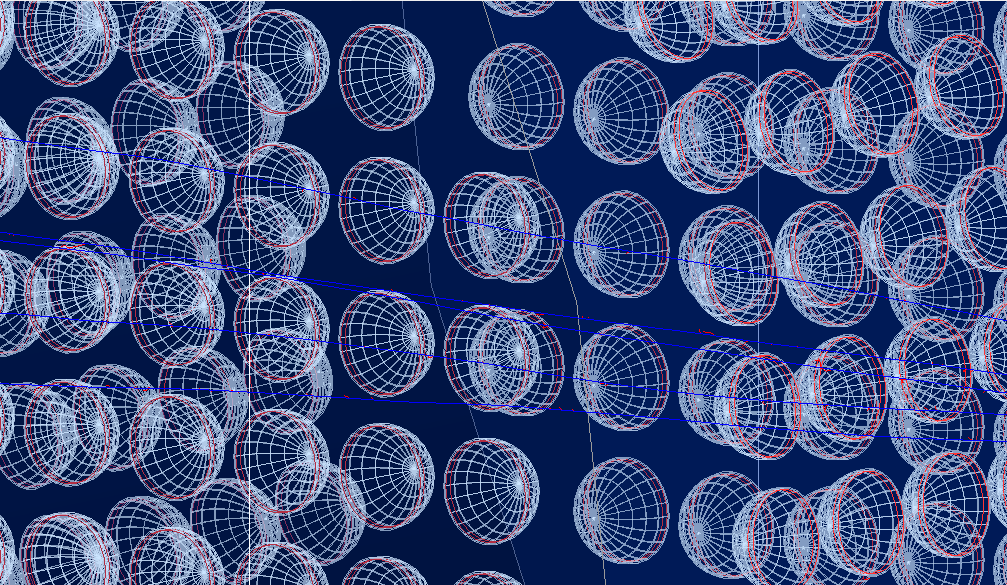
\includegraphics[width=0.82\textwidth]{../EvtDispl/Screenshot_from_2026-10-30_15-46-59.png}\caption{Event display snapshot 1.}\end{figure}
\begin{figure}[H]\centering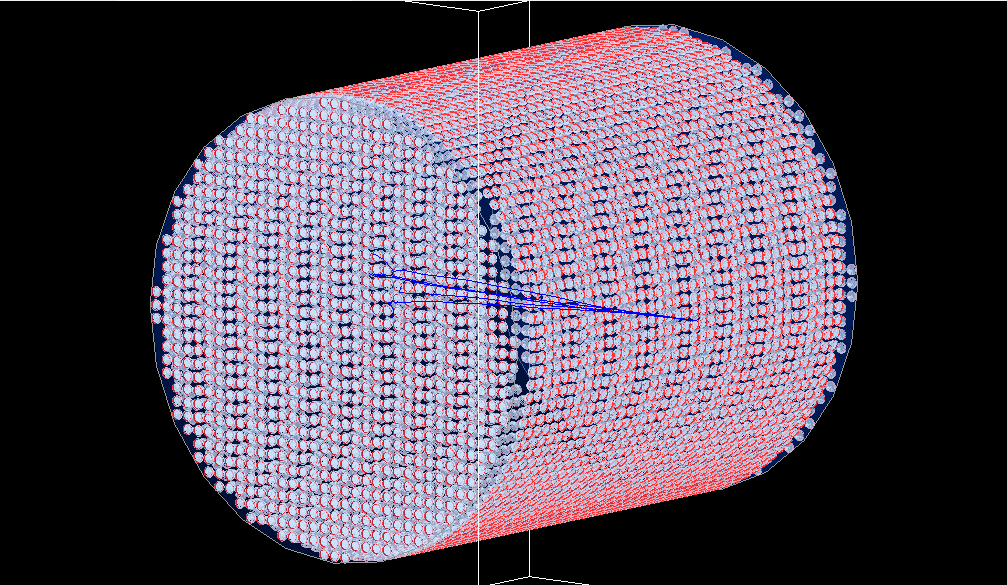
\includegraphics[width=0.82\textwidth]{../EvtDispl/Screenshot_from_2026-10-30_15-47-03.png}\caption{Event display snapshot 2.}\end{figure}
\begin{figure}[H]\centering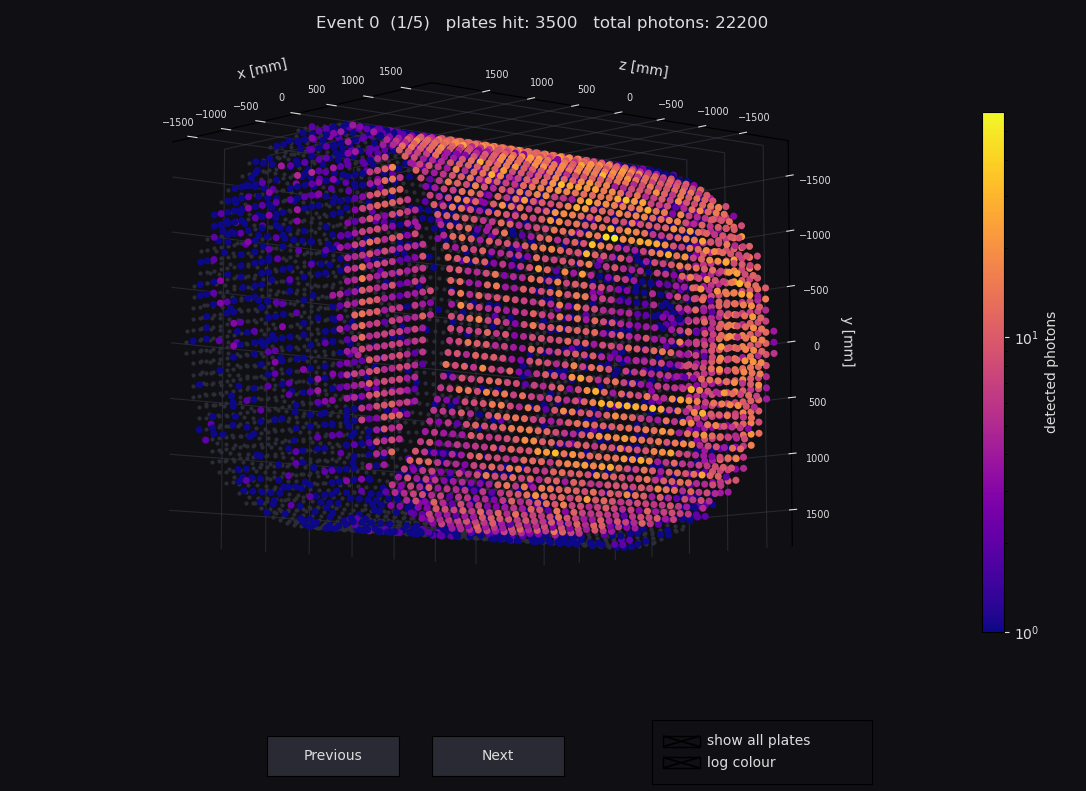
\includegraphics[width=0.82\textwidth]{../EvtDispl/Screenshot_from_2026-10-30_15-48-08.png}\caption{Event display snapshot 3.}\end{figure}
\begin{figure}[H]\centering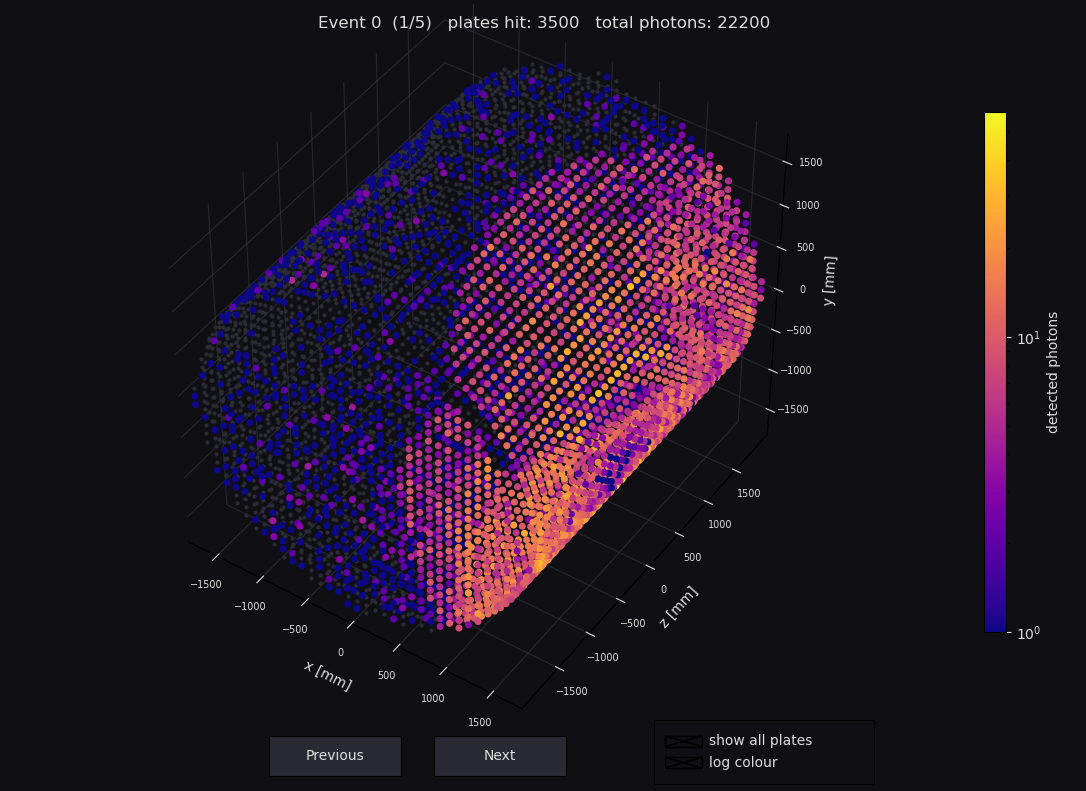
\includegraphics[width=0.82\textwidth]{../EvtDispl/Screenshot_from_2026-10-30_15-49-51.png}\caption{Event display snapshot 4.}\end{figure}
\begin{figure}[H]\centering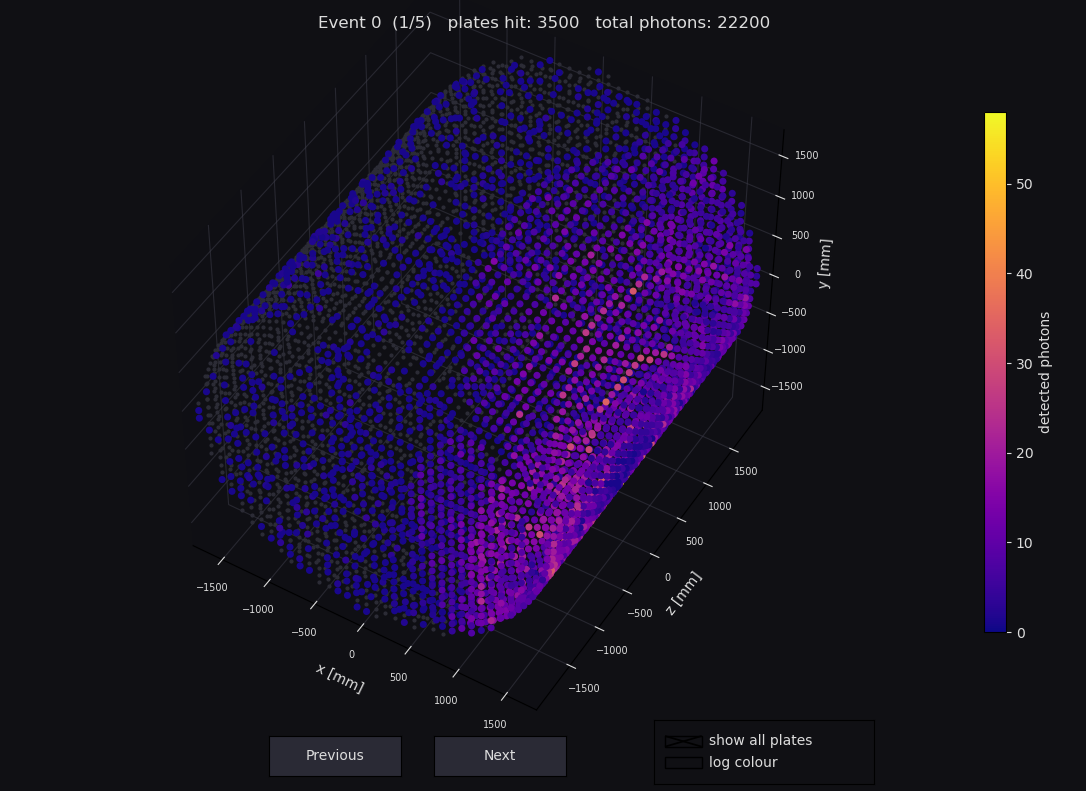
\includegraphics[width=0.82\textwidth]{../EvtDispl/Screenshot_from_2026-10-30_15-50-15.png}\caption{Event display snapshot 5.}\end{figure}

\subsection{Simulation and analysis screenshots (\texttt{Screenshots/})}
\begin{figure}[H]\centering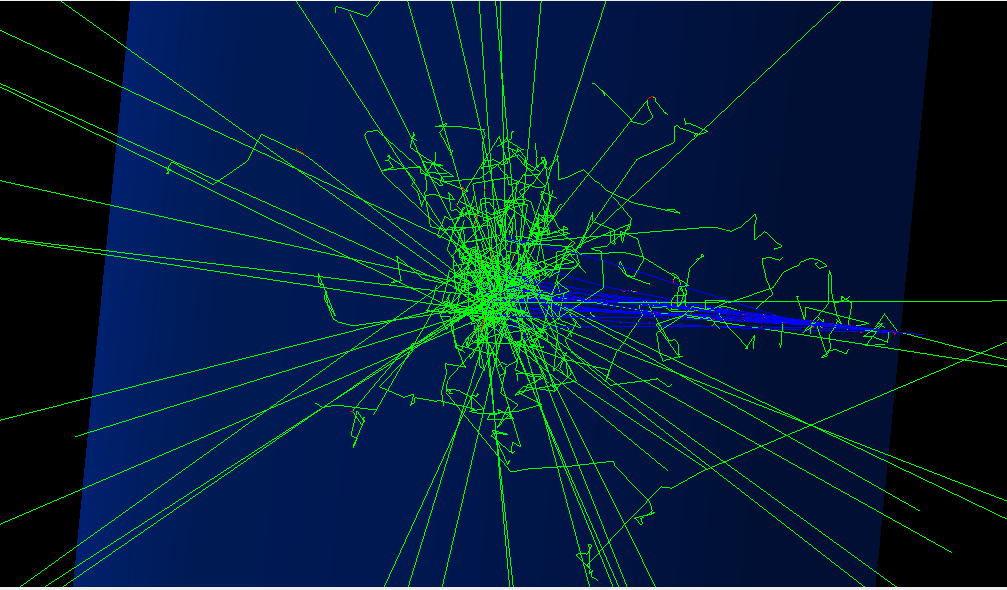
\includegraphics[width=0.82\textwidth]{../Screenshots/Screenshot_from_2026-10-24_15-01-46.png}\caption{Screenshot 1.}\end{figure}
\begin{figure}[H]\centering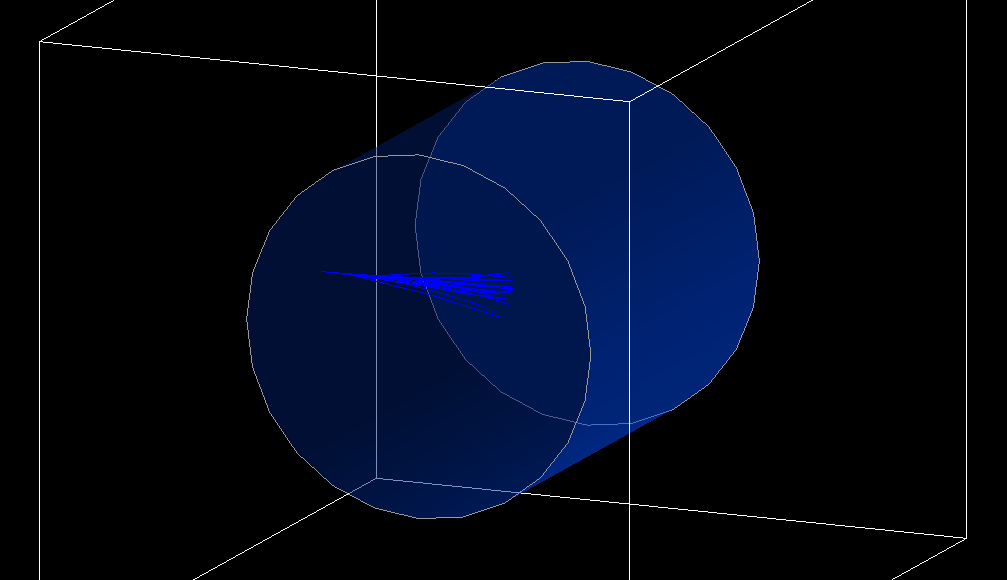
\includegraphics[width=0.82\textwidth]{../Screenshots/Screenshot_from_2026-10-24_15-11-40.png}\caption{Screenshot 2.}\end{figure}
\begin{figure}[H]\centering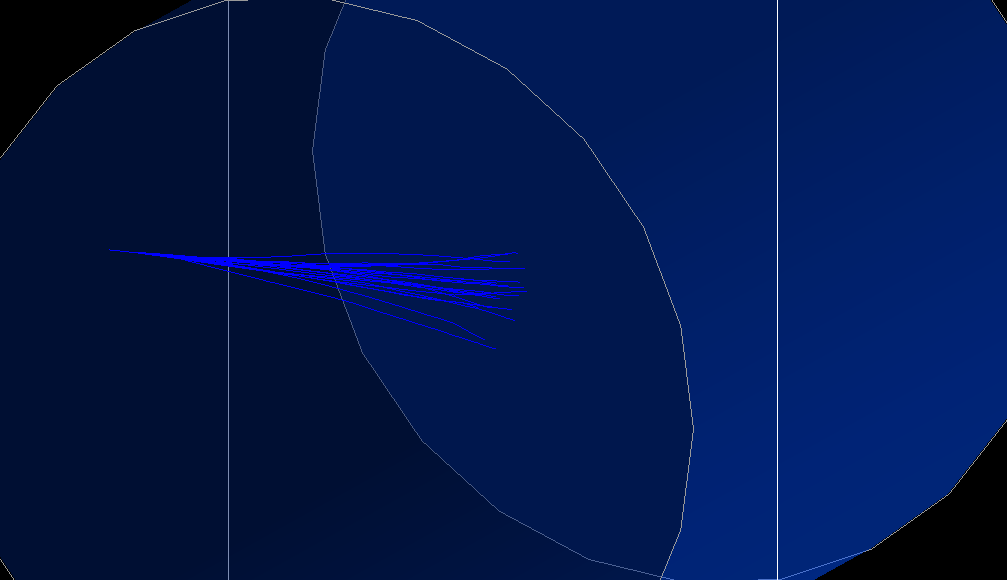
\includegraphics[width=0.82\textwidth]{../Screenshots/Screenshot_from_2026-10-24_15-11-45.png}\caption{Screenshot 3.}\end{figure}
\begin{figure}[H]\centering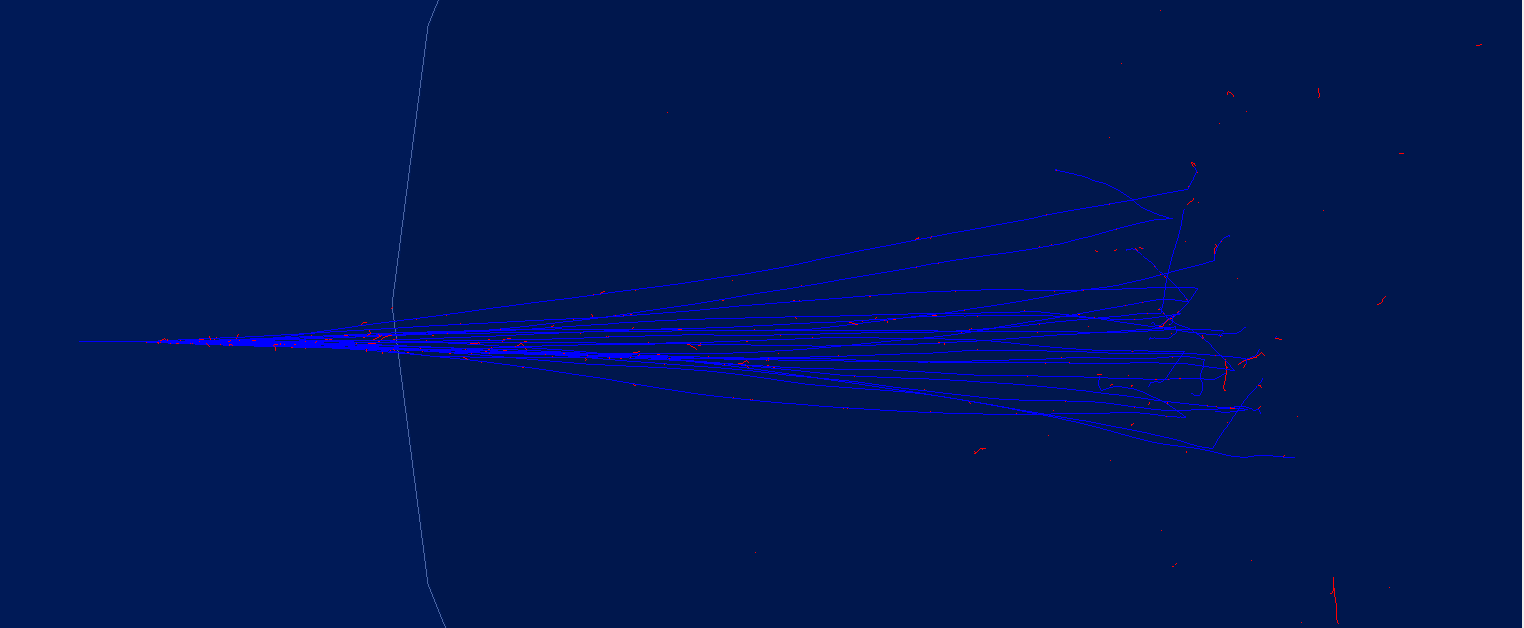
\includegraphics[width=0.82\textwidth]{../Screenshots/Screenshot_from_2026-10-25_11-50-18.png}\caption{Screenshot 4.}\end{figure}
\begin{figure}[H]\centering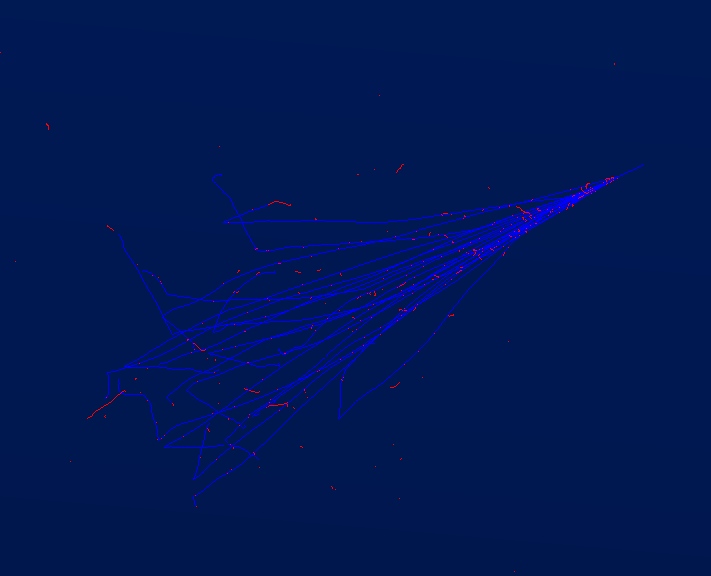
\includegraphics[width=0.82\textwidth]{../Screenshots/Screenshot_from_2026-10-25_11-50-39.png}\caption{Screenshot 5.}\end{figure}
\begin{figure}[H]\centering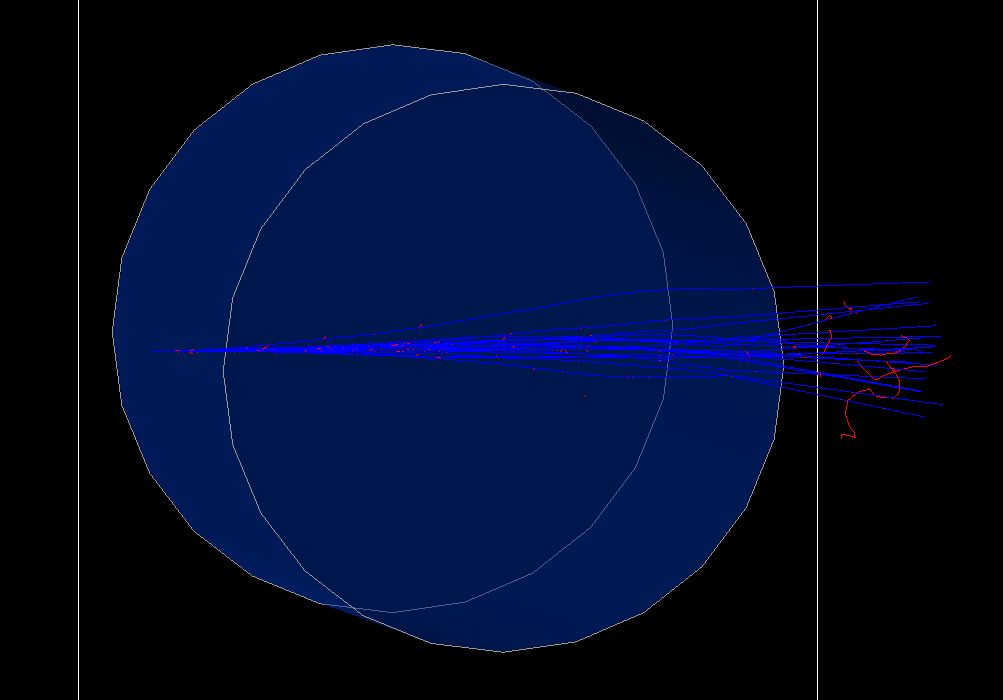
\includegraphics[width=0.82\textwidth]{../Screenshots/Screenshot_from_2026-10-25_11-52-45.png}\caption{Screenshot 6.}\end{figure}
\begin{figure}[H]\centering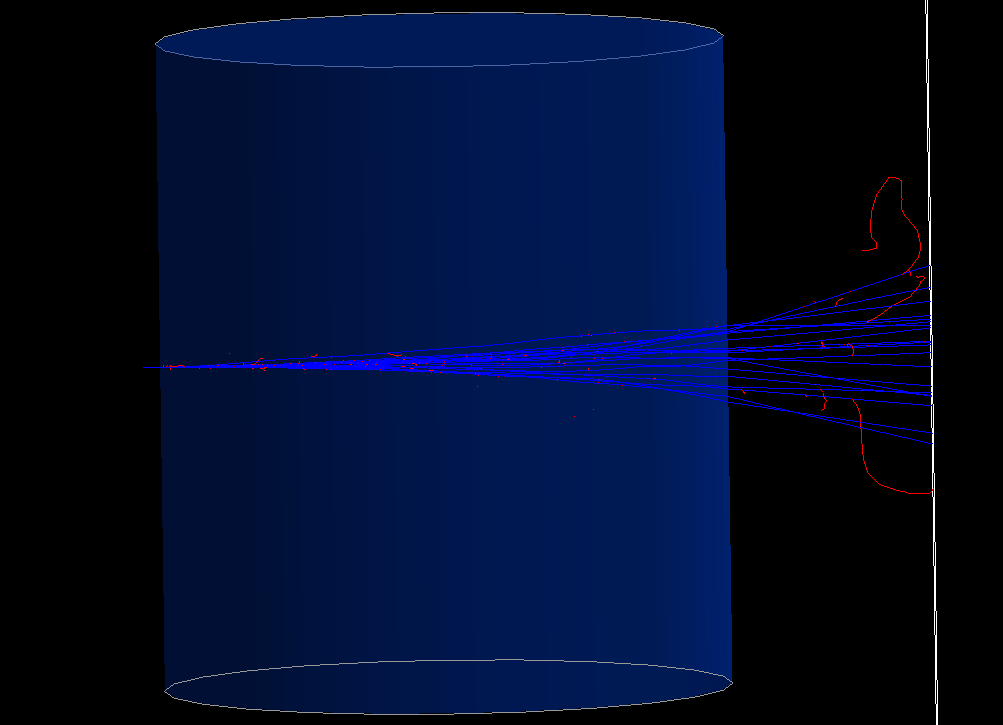
\includegraphics[width=0.82\textwidth]{../Screenshots/Screenshot_from_2026-10-25_11-53-16.png}\caption{Screenshot 7.}\end{figure}
\begin{figure}[H]\centering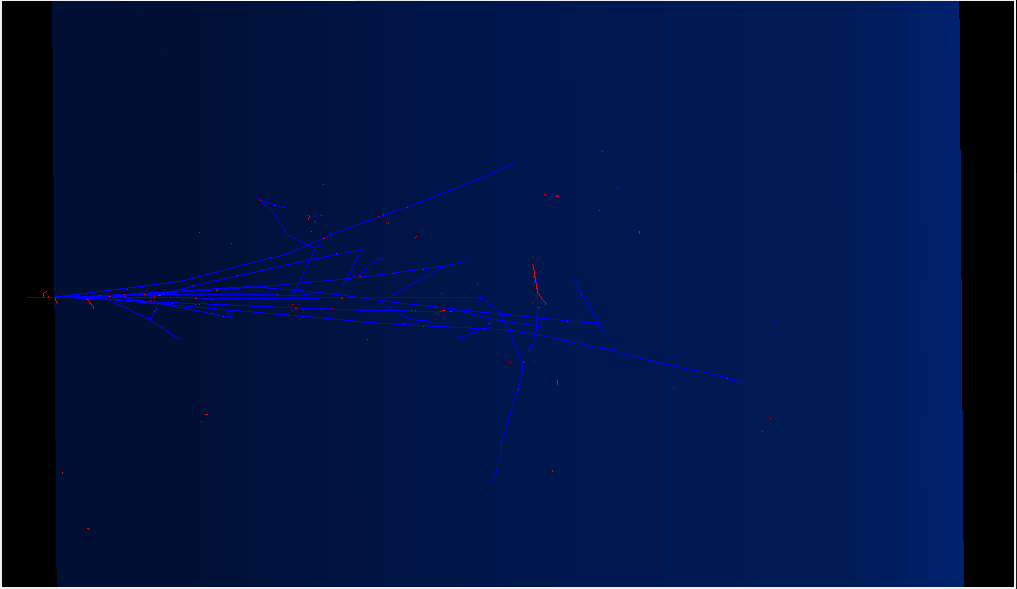
\includegraphics[width=0.82\textwidth]{../Screenshots/Screenshot_from_2026-10-30_09-00-12.png}\caption{Screenshot 8.}\end{figure}
\begin{figure}[H]\centering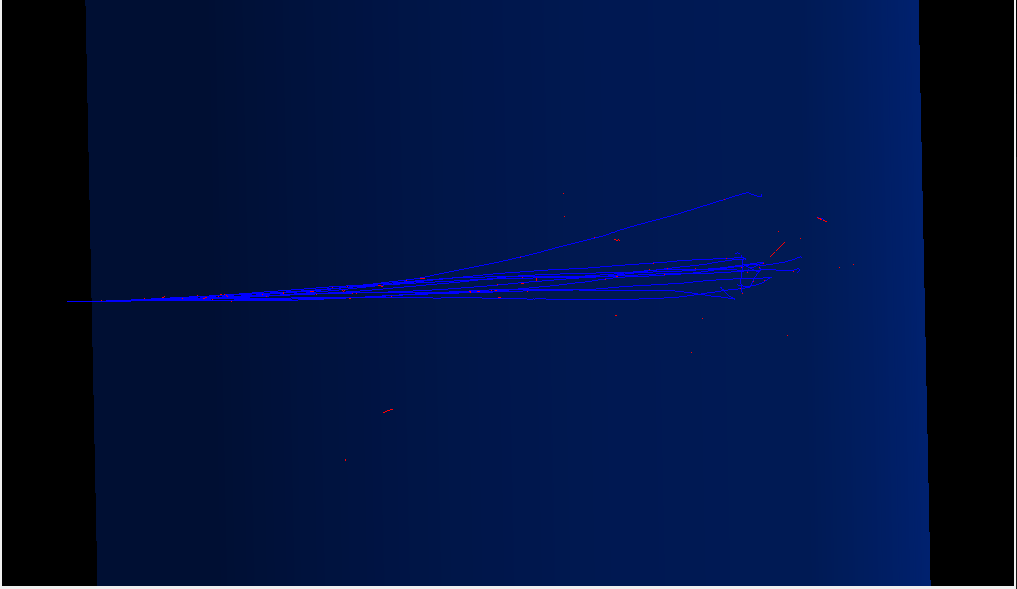
\includegraphics[width=0.82\textwidth]{../Screenshots/Screenshot_from_2026-10-30_09-00-46.png}\caption{Screenshot 9.}\end{figure}
\begin{figure}[H]\centering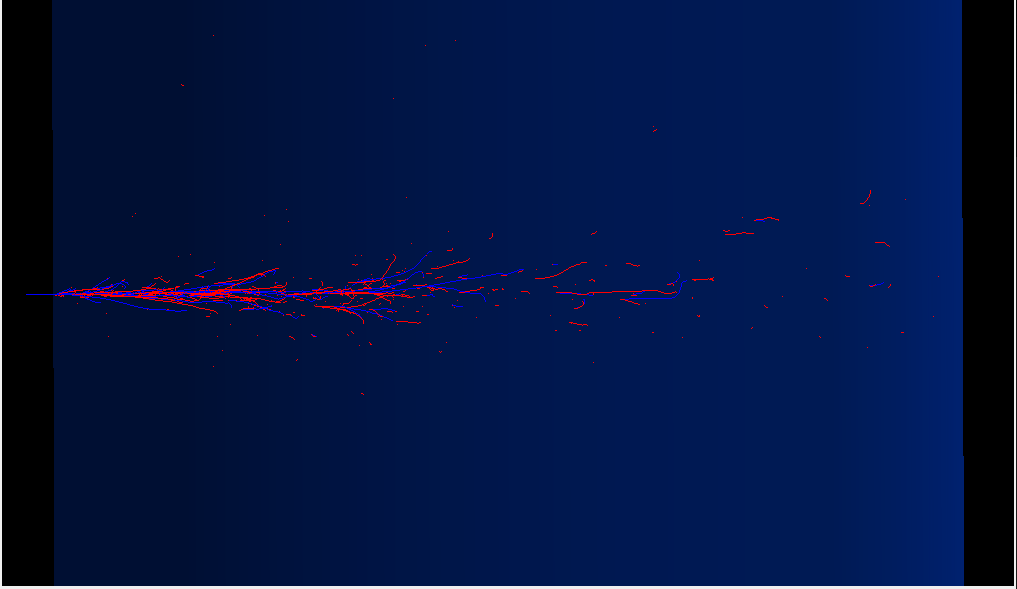
\includegraphics[width=0.82\textwidth]{../Screenshots/Screenshot_from_2026-10-30_09-01-35.png}\caption{Screenshot 10.}\end{figure}

\end{document}
